\documentclass[dvisvgm]{standalone}
\usepackage{tikz}
\usepackage{amsmath}
\usepackage{amsfonts}

\begin{document}
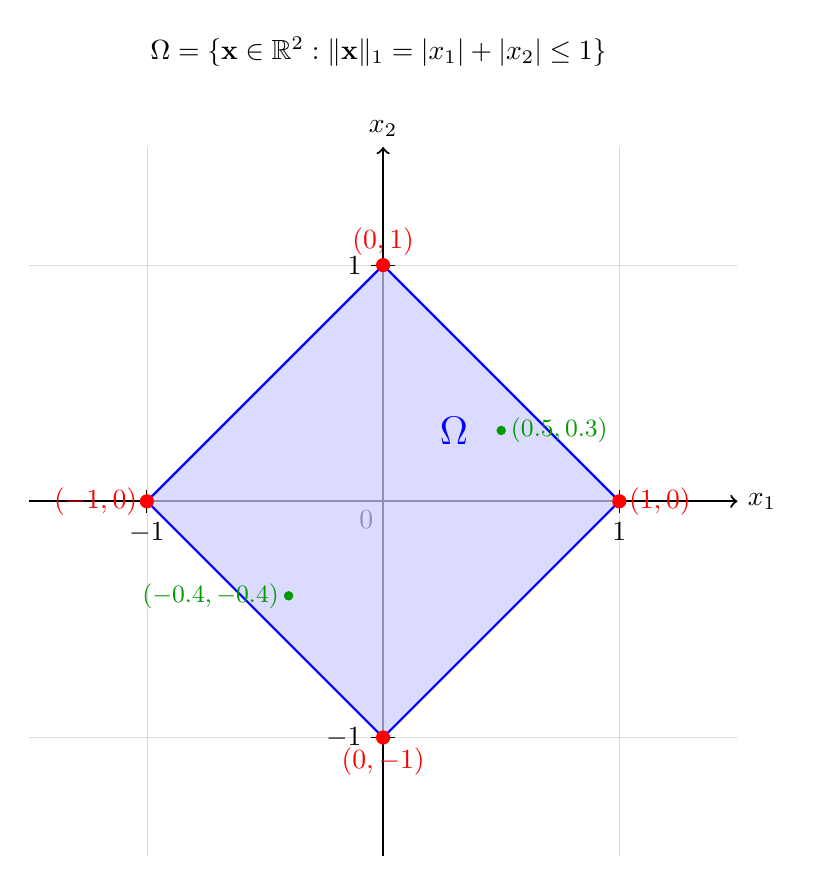
\begin{tikzpicture}[scale=3]
    % Grid
    \draw[help lines, gray!30] (-1.5,-1.5) grid (1.5,1.5);
    
    % Axes
    \draw[thick,->] (-1.5,0) -- (1.5,0) node[right] {$x_1$};
    \draw[thick,->] (0,-1.5) -- (0,1.5) node[above] {$x_2$};
    
    % Origin
    \node[below left] at (0,0) {$0$};
    
    % Tick marks
    \foreach \x in {-1,1} {
        \draw (\x,0.05) -- (\x,-0.05) node[below] {$\x$};
        \draw (0.05,\x) -- (-0.05,\x) node[left] {$\x$};
    }
    
    % L1-ball (diamond shape)
    \fill[blue!20, opacity=0.7] (1,0) -- (0,1) -- (-1,0) -- (0,-1) -- cycle;
    \draw[thick, blue] (1,0) -- (0,1) -- (-1,0) -- (0,-1) -- cycle;
    
    % Vertices of the diamond
    \fill[red] (1,0) circle (0.03) node[right] {$(1,0)$};
    \fill[red] (0,1) circle (0.03) node[above] {$(0,1)$};
    \fill[red] (-1,0) circle (0.03) node[left] {$(-1,0)$};
    \fill[red] (0,-1) circle (0.03) node[below] {$(0,-1)$};
    
    % Label for the region
    \node[blue, font=\Large] at (0.3,0.3) {$\Omega$};
    
    % Constraint equation
    \node[above, align=center] at (0,1.8) {
        $\Omega = \{\mathbf{x} \in \mathbb{R}^2 : \|\mathbf{x}\|_1 = |x_1| + |x_2| \leq 1\}$
    };
    
    % Example points
    \fill[green!60!black] (0.5,0.3) circle (0.02);
    \node[green!60!black, right] at (0.5,0.3) {\small $(0.5,0.3)$};
    
    \fill[green!60!black] (-0.4,-0.4) circle (0.02);
    \node[green!60!black, left] at (-0.4,-0.4) {\small $(-0.4,-0.4)$};
    
\end{tikzpicture}
\end{document}
